\documentclass[a4paper,11pt]{article}

\usepackage[UKenglish]{babel}
\usepackage{mathtools,amssymb,amsthm}
\usepackage{adjustbox,graphicx, caption}
\usepackage{hyperref}
\usepackage[margin=1in]{geometry}% Just for this example

% ========= Theorem-like environments =========
% These lines define theorem-like environments.
% See https://www.overleaf.com/learn/latex/theorems_and_proofs
\theoremstyle{definition}
\newtheorem{defn}{Definition}[section] % <--- for definitions
\newtheorem{theorem}[defn]{Theorem} % <--- modified
\newtheorem{prop}[defn]{Proposition}
\newtheorem{lemma}[defn]{Lemma}
\newtheorem{exmp}[defn]{Example}
\numberwithin{equation}{section} % <--- for equations
% =============================================

% ========= Bibliography =========
% These lines load the `biblatex' package
% and read in the list of references from
% References.bib - take a look.
%
% To generate References.bib, I recommend https://www.mybib.com/
% rather than trying to write the .bib file yourself.
%
\usepackage[]{csquotes, biblatex}
\addbibresource{References.bib}
% ================================

\title{Mandelbrot and Julia Sets}
\author{Gleb Sokolovski, s2015488}

\begin{document}
\maketitle

\section{Introduction}

Fractals are mathematical objects that display self-similarity, meaning that they look similar at different levels of magnification. Mandelbrot and Julia sets are two famous examples of fractals, both of which are generated by iterations of complex functions. In this paper, we will explore the mathematics behind these fractals and their connection.

\section{Julia Sets}

We begin by defining what's known as a filled-in Julia set. A reminder that the Reimann sphere $\mathbb{C}^*$ is the defined as the extended complex plane such that $\mathbb{C}^* = \mathbb{C} \cup \{ \infty \}$

\begin{defn}
    Let $c \in \mathbb{C}^{*}$ be a complex number on the Reimann sphere. For each point $z_0$ of the plane, we generate a sequence that satisfies the iteration :
    \begin{equation}
        z_{n+1} = z_n^2 + c.\label{eq:1}
    \end{equation}
    We define a set of $z_0$'s for which the sequence diverges to infinity as the filled-in Julia set. And we denote it as $K_C$.
\end{defn}


Following this, we arrive at the following defintion.

\begin{defn}
     Julia set $J_C$ is the boundary of the filled-in set (the set of "exceptional points").
\end{defn}


\begin{prop}
    Let $z_n$ be an element of the sequence $z_{n+1} = z_n^2 + c$. If $z_n$ is farther than 2 from the origin, then successive iterates will grow without bound.
\end{prop}
\begin{proof}
    For a complex number $z_n = x_n + i \cdot y_n$, we define the absolute value as $|z_n| = \sqrt{(x_n^2 + y_n^2)}$. So we want to show if some $z_n$ satisfies $|z_n| > \max (2, |c|)$, then the sequence $z_n, z_{n+1},...$ will diverge to infinity. 

    Suppose $|z_n| > \max (2, |c|)$. Then we can write (\ref{eq:1}) as 
    \begin{center}
        $|z_n| = 2 + \epsilon$,
    \end{center}
    for some $\epsilon > 0$. And since $|z_n^2| = |z_n^2 + c - c| \le |z_n^2 + c| + |c|$ due to triangle inequality, we can say that
    \begin{align*}
        |z_n^2 + c| &\ge |z_n^2| - |c| = |z_n|^2 - |c| \\
        &> |z_n|^2 - |z_n| (because |z_n| > |c|) \\
        &= (|z_n| - 1)\cdot|z_n| = (1 + \epsilon)\cdot|z_n| \\
    \end{align*}

    That is, $|z_{n+1}| > (1 + \epsilon)\cdot|z_n|$. Iterating, $|z_{n+k}| > (1 + \epsilon)^k\cdot|z_n|$.

    Now observe that if $|c| > 2$, then (noting $|c + 1| > 1$ because $|c| > 2$)
    \begin{align*}
            z_0 &= 0 \\
            z_1 &= c \\
            z_2 &= c_2 + c = c\cdot(c + 1) \\
            \rightarrow |z_2| &= |c|\cdot|c + 1| > |c|.
    \end{align*} 
    
\end{proof}


\begin{exmp}
    If we paint the sequence produce by $z_0$ at its center that doesn't diverge to infinity in black colour, and otherwise we paint the pixel a colour determined by how quickly sequence gets further than 2 from the origin (hence diverges), we get interesting "fractals", like the one at Figures \ref{fig:Julia_ex_1} and \ref{fig:Julia_ex_2}.
\end{exmp}

\begin{figure}[h]
    \centering
    \begin{minipage}{.5\textwidth}
        \centering
        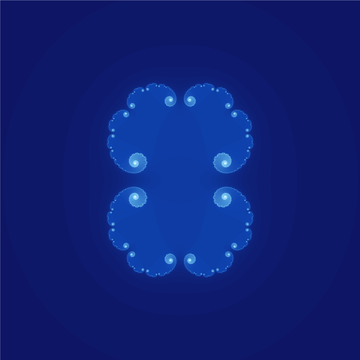
\includegraphics[width=.5\linewidth]{figures/Julia_0.285_0.png}
        \caption[width=.2\textwidth]{Julia set for $f_c$, $c =  0.285 + 0i$ \cite{julia-sets-examples}}
        \label{fig:Julia_ex_1}
    \end{minipage}%
    \begin{minipage}{.5\textwidth}
        \centering
        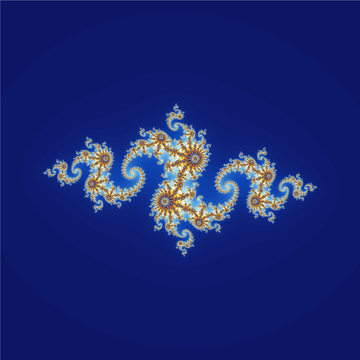
\includegraphics[width=.5\linewidth]{figures/Julia_-0.8_0.156.png}
        \caption[width=.2\textwidth]{Julia set for $f_c$, $c = -0.8 + 0.156i$ \cite{julia-sets-examples}}
        \label{fig:Julia_ex_2}
    \end{minipage}
\end{figure}



Let's now look at the two different types of Julia sets.

\begin{defn}[\cite{defn-of-fatou-sets-dust}]
    There are two types of Julia sets: connected sets - also known as Fatou Sets - and Cantor sets - also known as Fatou Duct.
    The Fatou set is the set of points in the complex plane where the Julia set is locally connected. More precisely, a point z in the Fatou set of a Julia set J is said to be locally connected if there exists a neighborhood U of z such that the set of all points in U that belong to J is connected.
    While the Cantor set is a subset C of the Fatou set F of a Julia set J that satisfies the following properties:
    \begin{enumerate}
        \item C is compact and connected.
        \item C has no isolated points.
        \item C is perfect, meaning that every point of C is a limit point of C.
        \item C is nowhere dense, meaning that its closure has empty interior.
        \item C has a self-similar structure, meaning that it can be expressed as the union of finitely many copies of itself, each of which is scaled by a fixed factor and translated to a different location.
    \end{enumerate}

\end{defn}

\begin{exmp}
    Consider the complex quadratic polynomial $f(z) = z^2 - 1$. The Julia set J of this polynomial is the set of all points in the complex plane that have chaotic behavior under iterations of f.

    The Fatou set F of this Julia set consists of all points in the complex plane that have stable behavior under iterations of f.

    As for an example of a Cantor set (or Fatou dust) for this Julia set, we could consider the set of points that are attracted to a repelling periodic orbit of f. Specifically, let p be the fixed point of f given by $p = (1 + \sqrt{5})/2$, and let C be the set of all points in the complex plane that converge to p under iterations of f. This set C is a Cantor set.
\end{exmp}

We just need one more definition to set us up perfectly for the important theorem. It's the definition many have heard of - but I will put in it just in case you haven't.

\begin{defn}
    Critical points are the points in the complex plane where the derivative of a function is zero or undefined. In other words:
    \begin{center}
        CPs$( f(z) )$ = $\{ z : f'(z) = 0~||~f'(z) $ is undefined $ \}$.
    \end{center}
    
\end{defn}

\begin{theorem}[Dichotomy Theorem]
    For any polynomial f, if all the critical points of f belong to $K_f$, then $J_f$ is connected and if none of the critical points of f belong to $K_f$, then $J_f$ is a Cantor set.
\end{theorem}
\begin{proof}
    To prove these statements, we need to use the theory of complex dynamics, which is a branch of mathematics that studies the iteration of complex functions. In particular, we will need to use the theory of iteration of polynomials, which is a special case of complex dynamics.
    First, we define the filled-in Julia set $K_f$ of a polynomial f to be the set of points z in the complex plane such that the iterates ${f^n(z)}_n = 0^{\infty}$ are bounded. That is,
    \begin{center}
        $K_f = \{ z : {f^n(z)}_n = 0^{\infty} $ is bounded $ \}$.
    \end{center}
    The Julia set $J_f$ is then defined as the boundary of $K_f$, that is, $J_f = \partial K_f$.
    Now, we can prove the two statements:
    \begin{enumerate}
        \item If all the critical points of f belong to $K_f$, then $J_f$ is connected.
        \item If none of the critical points of f belong to $K_f$, then $J_f$ is a Cantor set.
    \end{enumerate}
    I will not get into the proof of them, but you can read about it here \cite{dichotomy}.

\end{proof}



\printbibliography

\end{document}